\documentclass[11pt,a4paper]{article}

\usepackage[margin=1in]{geometry}
\usepackage{graphicx}
\usepackage{booktabs}
\usepackage{array}
\usepackage{longtable}
\usepackage{caption}
\usepackage{subcaption}
\usepackage{xcolor}
\usepackage{listings}
\usepackage{amsmath}
\usepackage{enumitem}
\usepackage{fancyhdr}
\usepackage{titlesec}
\usepackage[hidelinks]{hyperref}

\definecolor{codebg}{RGB}{245,245,245}
\definecolor{codekw}{RGB}{0,80,150}
\definecolor{codecomment}{RGB}{110,110,110}
\definecolor{codestring}{RGB}{140,20,20}

\lstset{
  backgroundcolor=\color{codebg},
  basicstyle=\ttfamily\small,
  keywordstyle=\color{codekw}\bfseries,
  commentstyle=\color{codecomment}\itshape,
  stringstyle=\color{codestring},
  showstringspaces=false,
  breaklines=true,
  frame=single,
  rulecolor=\color{gray!40},
  numbers=left,
  numberstyle=\tiny\color{gray},
  xleftmargin=1.8em,
  language=Python
}

\titleformat{\section}{\normalfont\Large\bfseries}{\thesection}{1em}{}
\titleformat{\subsection}{\normalfont\large\bfseries}{\thesubsection}{1em}{}

\pagestyle{fancy}
\fancyhf{}
\fancyhead[L]{ICS1512 -- Machine Learning Algorithms Laboratory}
\fancyhead[R]{Experiment 7}
\fancyfoot[C]{\thepage}
\renewcommand{\headrulewidth}{0.4pt}

\title{}
\date{}

\begin{document}

% ---------------- Title Page ----------------
\begin{titlepage}
\centering
\vspace*{1cm}
{\Large\bfseries Sri Sivasubramaniya Nadar College of Engineering, Chennai\par}
\vspace{0.2cm}
{\normalsize (An Autonomous Institution Affiliated to Anna University)\par}
\vspace{1.2cm}

{\Large\bfseries Machine Learning Algorithms Laboratory\par}
\vspace{0.3cm}
{\large ICS1512\par}
\vspace{1.5cm}

\begin{tabular}{|p{5.5cm}|p{7cm}|}
\hline
Degree \& Branch & M.Tech (Integrated) Computer Science \& Engineering \\
\hline
Semester & V \\
\hline
Academic Year & 2026--2027 (Odd) \\
\hline
Batch & 2024--2029 \\
\hline
\end{tabular}

\vspace{1.8cm}
{\Large\bfseries Experiment 7\par}
\vspace{0.3cm}
{\large Dimensionality Reduction and Model Evaluation (With and Without PCA)\footnote{\textbf{GitHub Repository: }\url{https://github.com/VijayaraaghavanKS/ML}}\par}
\vspace{2.5cm}

\begin{tabular}{ll}
Submitted by: & \textbf{Vijayaraaghavan K S} \\[4pt]
Register Number: & \textbf{3122247001066} \\[4pt]
Year: & III Year \\[4pt]
Programme: & M.Tech Integrated, CSE \\[4pt]
Faculty: & Dr. Poreddy Ajay Kumar Reddy \\[4pt]
\end{tabular}

\vfill
\end{titlepage}

\tableofcontents
\newpage

% ==========================================================
\section{Aim and Objective}
To study the effect of Principal Component Analysis (PCA) on classifier performance by training and hyperparameter-tuning ten models -- SVM, Naive Bayes, KNN, Logistic Regression, Decision Tree, Random Forest, AdaBoost, Gradient Boosting, XGBoost, and a Stacked Ensemble -- on the Wisconsin Diagnostic Breast Cancer dataset, once on the original 30-feature space and once on a PCA-reduced feature space, using 5-fold cross-validation throughout, and to determine for which model families PCA helps, hurts, or makes no practical difference.

% ==========================================================
\section{Problem Statement}
The input is the same 30-dimensional vector of nuclear-morphology measurements used in Experiments 5 and 6; the output is a binary diagnosis, malignant or benign. This experiment asks a question orthogonal to Experiments 5 and 6: rather than comparing model families to each other on a fixed feature space, it fixes the model family and asks whether compressing the feature space with PCA (10 principal components instead of 30 standardized features, chosen to retain 95\% of the variance) changes the answer -- and whether that change is the same for every model, or specific to how each model uses the feature space geometrically.

% ==========================================================
\section{Theory}

\subsection{Principal Component Analysis (PCA)}
PCA is an unsupervised linear transformation that projects standardized features onto a new set of orthogonal axes (principal components), ordered so that the first component captures the most variance in the data, the second captures the most variance orthogonal to the first, and so on. Keeping only the leading components needed to reach a target cumulative explained-variance ratio compresses the feature space while discarding the directions that carry the least information, which also removes the multicollinearity that comes from having many correlated raw features (44 feature pairs here exceed 0.80 Pearson correlation, as already reported in Experiments 5 and 6).

\subsection{Why PCA's Effect is Model-Dependent}
Distance-based and margin-based models (KNN, SVM, Logistic Regression) compute their decisions directly from distances or dot products in feature space, so redundant, correlated features can distort those geometric computations; PCA's decorrelation and dimensionality reduction tends to help these models, or at least does not hurt them much, since the components it removes carry little independent signal. Tree-based models (Decision Tree, Random Forest, AdaBoost, Gradient Boosting, XGBoost) instead pick one informative feature to split on at a time and are largely indifferent to correlated features sitting alongside the one they choose; rotating the space into PCA components can actually make their job harder, since a single original feature with a clean, interpretable split threshold can get smeared across several PCA components that each carry only part of its signal. Stacking, since it combines the outputs of several base learners, should show an effect that is some blend of its base learners' individual sensitivities to PCA.

% ==========================================================
\section{Machine Learning Algorithms}

\subsection{Distance/Margin-Based Models}
\textbf{SVM} finds the maximum-margin hyperplane separating the two classes (optionally in a kernel-induced feature space); \textbf{KNN} classifies a point by majority vote among its $k$ nearest neighbors under a chosen distance metric; \textbf{Logistic Regression} fits a linear decision boundary by maximizing the likelihood of a sigmoid-transformed linear score. All three depend directly on distances or dot products between feature vectors, so the scale and correlation structure of the feature space matters to their decision boundary.

\subsection{Probabilistic Model}
\textbf{Naive Bayes} (Gaussian variant here) assumes each feature is conditionally independent of every other feature given the class, and multiplies per-feature class-conditional Gaussian densities to obtain a posterior. This independence assumption is directly violated by the 44 highly correlated feature pairs in the raw feature space; PCA's decorrelation should, in principle, make the independence assumption less wrong.

\subsection{Tree-Based and Ensemble Models}
\textbf{Decision Tree} recursively splits the feature space along single-feature thresholds chosen to maximize class purity; \textbf{Random Forest} bags many such trees over bootstrap samples and random feature subsets; \textbf{AdaBoost} and \textbf{Gradient Boosting} build trees sequentially, each correcting the previous ensemble's errors (via reweighting or gradient-residual fitting respectively); \textbf{XGBoost} is a regularized, second-order gradient-boosting implementation with the same sequential-correction principle but faster, more regularized tree construction. All five choose splits on individual features (whether raw or PCA components) rather than on distances, so their sensitivity to PCA comes only from whether the transformed features are as easy to split on as the original ones.

\subsection{Stacked Ensemble}
The Stacking model combines SVM, Random Forest, and Gradient Boosting as base learners (chosen as the three strongest models observed in Experiments 5 and 6's model families) with a Logistic Regression meta-learner trained on their cross-validated out-of-fold predictions, so it inherits some of each base learner's individual response to PCA while the meta-learner can partially compensate for any one base learner's degradation.

% ==========================================================
\section{Dataset}
This experiment reuses the same Wisconsin Diagnostic Breast Cancer dataset as Experiments 5 and 6 (569 samples, 30 numeric features, binary \texttt{diagnosis} label), loaded through scikit-learn's \texttt{load\_breast\_cancer} function and written out as a CSV so it flows through the same shared EDA pipeline used by Experiments 1--6. After the EDA pipeline's 80/20 stratified split, the working data is 455 training rows and 114 test rows across 30 features, with 357 benign and 212 malignant cases overall. The target was label-encoded to 0 (benign) / 1 (malignant) so that every model, including XGBoost (which requires integer class labels in the installed version), could be trained and evaluated through the same uniform pipeline.

% ==========================================================
\section{Preprocessing and Exploratory Data Analysis}
The EDA pipeline reports zero missing values and zero duplicate rows across all 569 samples, so no imputation or de-duplication was needed. Every feature is numeric and was standardized before modelling, which is also the necessary precondition for PCA (PCA is only meaningful on features of comparable scale). As in Experiments 5 and 6, 44 feature pairs exceed a 0.80 Pearson correlation, driven by near-deterministic relationships between radius, perimeter, and area at the mean/error/worst level -- this is exactly the kind of redundancy PCA is designed to compress away.

\begin{figure}[h]
\centering
\begin{subfigure}{0.48\textwidth}

\includegraphics[width=\linewidth]{experiment7_output/eda_reuse/plots/class_distribution.png}
\caption{Class distribution}
\end{subfigure}
\hfill
\begin{subfigure}{0.48\textwidth}

\includegraphics[width=\linewidth]{experiment7_output/eda_reuse/plots/correlation_heatmap.png}
\caption{Feature correlation heatmap}
\end{subfigure}
\caption{EDA diagnostics, reused from the shared pipeline.}
\end{figure}

% ==========================================================
\section{Experimental Setup}
\begin{table}[h]
\centering
\begin{tabular}{ll}
\toprule
Python Version & 3.14.5 \\
Scikit-Learn Version & 1.9.0 \\
XGBoost Version & 3.4.1 \\
IDE & Jupyter Notebook \\
Operating System & macOS (Darwin 25.5.0, arm64) \\
Hardware & Apple Silicon (arm64), local machine \\
\bottomrule
\end{tabular}
\caption{Software and hardware environment used to run this experiment.}
\end{table}

% ==========================================================
\section{PCA: Component Selection}
A full PCA was first fit on the 30 standardized training features to inspect the cumulative explained-variance curve, then the smallest number of components reaching a 95\% variance target was chosen.

\begin{table}[h]
\centering
\begin{tabular}{@{}lp{3.6cm}rp{5.2cm}@{}}
\toprule
Setting & Chosen Components / Variance Target & Explained Variance (\%) & Justification \\
\midrule
With-PCA & 10 components (target 95\%) & 95.21 & Smallest number of components whose cumulative explained variance reaches the 95\% target, chosen from the scree plot to compress 30 original features while retaining most information. \\
\bottomrule
\end{tabular}
\caption{PCA variance-explained summary.}
\end{table}

\begin{figure}[h]
\centering
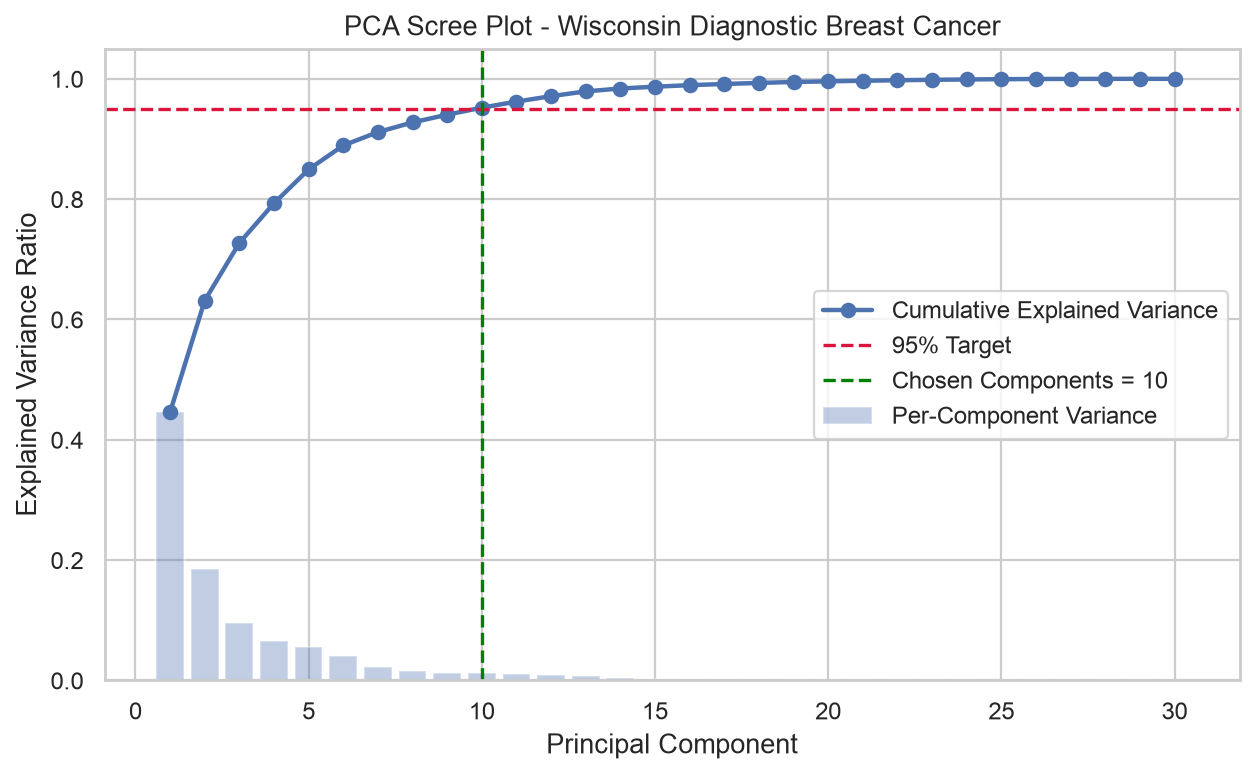
\includegraphics[width=0.72\linewidth]{experiment7_output/plots/pca_scree_plot.png}
\caption{PCA scree plot: per-component and cumulative explained variance, with the chosen 10-component cutoff marked.}
\end{figure}
The scree plot shows a steep drop after the first two or three components (which alone already explain a large majority of the variance, consistent with the dominant size/shape correlated feature groups identified during EDA), followed by a long, shallow tail. Ten components are needed to cross the 95\% cumulative variance line, compressing 30 features down by two-thirds while discarding only about 5\% of the total variance -- a favorable trade-off if PCA turns out to help the downstream models.

\begin{figure}[h]
\centering
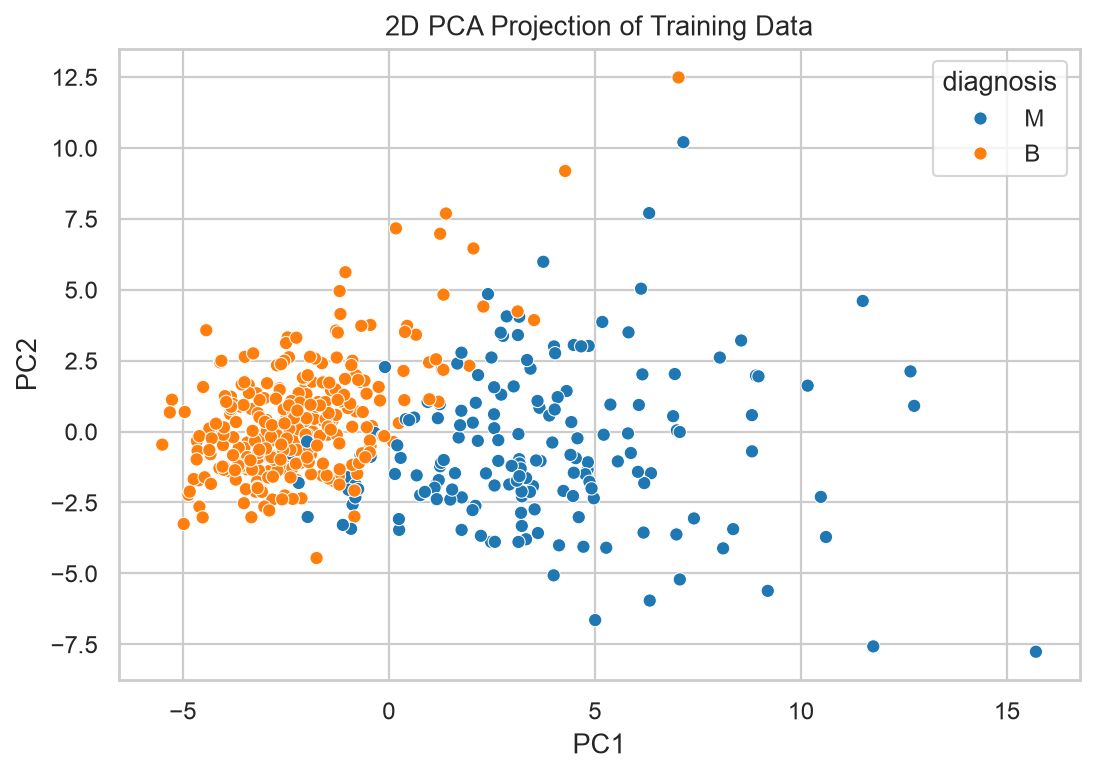
\includegraphics[width=0.6\linewidth]{experiment7_output/plots/pca_2d_projection_experiment7.png}
\caption{2D PCA projection of the training data (first two components only), colored by diagnosis.}
\end{figure}
Even in just two dimensions, the malignant and benign classes separate substantially, which foreshadows why several models (Decision Tree, XGBoost) show almost no accuracy change between the No-PCA and With-PCA settings -- most of the class-discriminating signal survives in a small number of leading components.

% ==========================================================
\section{Hyperparameter Grids}
The same hyperparameter grid was used for each model under both the No-PCA and With-PCA settings, so that any observed difference reflects the feature space rather than a different search budget.
\begin{lstlisting}
model_specs = {
    "SVM": (SVC(probability=True), {"kernel": ["linear", "rbf"], "C": [0.1, 1, 10], "gamma": ["scale", "auto"]}),
    "Naive Bayes": (GaussianNB(), {"var_smoothing": [1e-9, 1e-8, 1e-7, 1e-6]}),
    "KNN": (KNeighborsClassifier(), {"n_neighbors": [3, 5, 7, 9, 11], "weights": ["uniform", "distance"],
        "metric": ["euclidean", "manhattan"]}),
    "Logistic Regression": (LogisticRegression(max_iter=5000), {"C": [0.01, 0.1, 1, 10], "penalty": ["l2"]}),
    "Decision Tree": (DecisionTreeClassifier(), {"max_depth": [3, 5, 7, None], "min_samples_split": [2, 5, 10]}),
    "Random Forest": (RandomForestClassifier(), {"n_estimators": [100, 200], "max_depth": [5, 10, None],
        "min_samples_split": [2, 5]}),
    "AdaBoost": (AdaBoostClassifier(), {"n_estimators": [50, 100, 200], "learning_rate": [0.1, 0.5, 1.0]}),
    "Gradient Boosting": (GradientBoostingClassifier(), {"n_estimators": [100, 200], "learning_rate": [0.05, 0.1],
        "max_depth": [2, 3]}),
    "XGBoost": (XGBClassifier(eval_metric="logloss"), {"n_estimators": [100, 200], "learning_rate": [0.05, 0.1],
        "max_depth": [2, 3]}),
}
grid_search = GridSearchCV(estimator, param_grid, scoring={"accuracy": "accuracy", "f1": f1_scorer},
    refit="accuracy", cv=StratifiedKFold(n_splits=5, shuffle=True, random_state=42), n_jobs=-1)
\end{lstlisting}
Stacking used a lighter grid, \texttt{\{"final\_estimator\_\_C": [0.1, 1, 10]\}}, tuning only the meta-learner's regularization strength while its three base learners (SVM, Random Forest, Gradient Boosting) were reused from their own already-tuned configuration for that feature setting.

% ==========================================================
\section{Hyperparameter Tuning Results}
\begin{table}[h]
\centering
\small
\begin{tabular}{@{}p{2.7cm}p{5.3cm}p{5.3cm}@{}}
\toprule
Model & Best Parameters (No-PCA) & Best Parameters (With-PCA) \\
\midrule
SVM & \{C: 10, gamma: scale, kernel: rbf\} & \{C: 10, gamma: scale, kernel: rbf\} \\
Naive Bayes & \{var\_smoothing: 1e-09\} & \{var\_smoothing: 1e-09\} \\
KNN & \{metric: manhattan, n\_neighbors: 3, weights: uniform\} & \{metric: euclidean, n\_neighbors: 3, weights: uniform\} \\
Logistic Regression & \{C: 1, penalty: l2\} & \{C: 1, penalty: l2\} \\
Decision Tree & \{max\_depth: 7, min\_samples\_split: 2\} & \{max\_depth: 5, min\_samples\_split: 10\} \\
Random Forest & \{max\_depth: 5, min\_samples\_split: 2, n\_estimators: 100\} & \{max\_depth: 5, min\_samples\_split: 5, n\_estimators: 100\} \\
AdaBoost & \{learning\_rate: 0.5, n\_estimators: 100\} & \{learning\_rate: 0.5, n\_estimators: 100\} \\
Gradient Boosting & \{learning\_rate: 0.1, max\_depth: 2, n\_estimators: 200\} & \{learning\_rate: 0.1, max\_depth: 2, n\_estimators: 200\} \\
XGBoost & \{learning\_rate: 0.05, max\_depth: 2, n\_estimators: 200\} & \{learning\_rate: 0.1, max\_depth: 3, n\_estimators: 200\} \\
Stacking & \{final\_estimator\_\_C: 10\} & \{final\_estimator\_\_C: 10\} \\
\bottomrule
\end{tabular}
\caption{GridSearchCV best hyperparameters for every model, No-PCA vs.\ With-PCA.}
\end{table}
Most models land on the same or a very similar hyperparameter configuration in both feature spaces -- SVM, Naive Bayes, AdaBoost, Gradient Boosting, and Stacking all pick identical or near-identical settings -- which suggests the search grids were wide enough that PCA did not force a qualitatively different model complexity, only a different feature representation.

% ==========================================================
\section{5-Fold Cross-Validation Results}
\begin{table}[h]
\centering
\small
\begin{tabular}{@{}lrrrrrrr@{}}
\toprule
Model & Fold 1 & Fold 2 & Fold 3 & Fold 4 & Fold 5 & Avg (No-PCA) & Avg (With-PCA) \\
\midrule
SVM & 0.967 & 0.989 & 0.967 & 0.978 & 0.978 & 0.9758 & 0.9714 \\
Naive Bayes & 0.956 & 0.978 & 0.912 & 0.912 & 0.934 & 0.9385 & 0.9121 \\
KNN & 0.967 & 1.000 & 0.967 & 0.956 & 0.989 & 0.9758 & 0.9714 \\
Logistic Regression & 0.956 & 0.967 & 1.000 & 0.978 & 0.967 & 0.9736 & 0.9758 \\
Decision Tree & 0.890 & 0.967 & 0.890 & 0.912 & 0.956 & 0.9231 & 0.9385 \\
Random Forest & 0.967 & 1.000 & 0.945 & 0.945 & 0.978 & 0.9670 & 0.9582 \\
AdaBoost & 0.956 & 0.967 & 0.967 & 0.978 & 0.989 & 0.9714 & 0.9714 \\
Gradient Boosting & 0.967 & 0.978 & 0.967 & 0.967 & 0.989 & 0.9736 & 0.9582 \\
XGBoost & 0.967 & 0.978 & 0.967 & 0.967 & 0.989 & 0.9736 & 0.9736 \\
Stacking & 0.956 & 0.989 & 0.978 & 0.978 & 0.989 & 0.9780 & 0.9714 \\
\bottomrule
\end{tabular}
\caption{5-fold cross-validation accuracy (No-PCA fold values shown; Avg columns are each setting's best GridSearchCV mean CV accuracy).}
\end{table}

\begin{figure}[h]
\centering
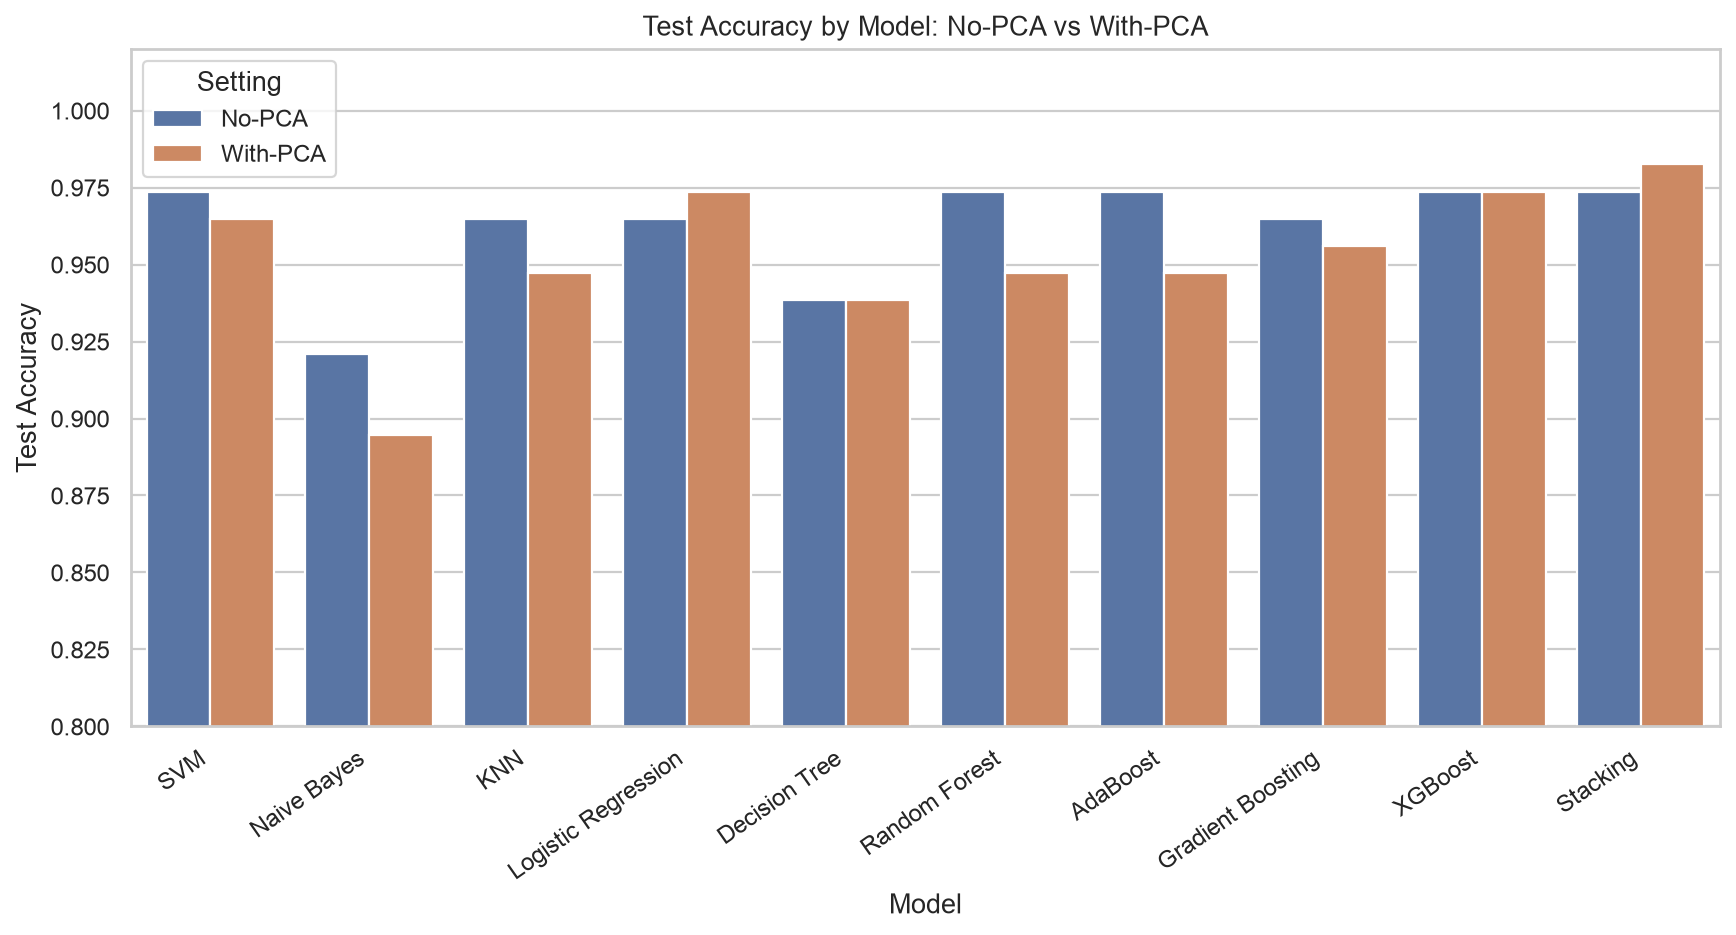
\includegraphics[width=0.8\linewidth]{experiment7_output/plots/accuracy_comparison_no_pca_vs_pca.png}
\caption{Test-set accuracy for all ten models, No-PCA vs.\ With-PCA.}
\end{figure}
Stacking has the highest No-PCA cross-validated accuracy (0.9780) of any model, while Naive Bayes is clearly the weakest performer in both settings (0.9385 No-PCA, 0.9121 With-PCA) -- a direct consequence of its independence assumption being most violated by the raw, highly correlated feature set, and only partially repaired once PCA decorrelates the input.

% ==========================================================
\section{Test-Set Performance Comparison}
\begin{table}[h]
\centering
\small
\begin{tabular}{@{}llrrrrr@{}}
\toprule
Model & Setting & Accuracy & Precision & Recall & F1 & ROC-AUC \\
\midrule
SVM & No-PCA & 0.9737 & 1.0000 & 0.9286 & 0.9630 & 0.9927 \\
SVM & With-PCA & 0.9649 & 0.9750 & 0.9286 & 0.9512 & 0.9904 \\
Naive Bayes & No-PCA & 0.9211 & 0.9231 & 0.8571 & 0.8889 & 0.9891 \\
Naive Bayes & With-PCA & 0.8947 & 0.8571 & 0.8571 & 0.8571 & 0.9613 \\
KNN & No-PCA & 0.9649 & 1.0000 & 0.9048 & 0.9500 & 0.9735 \\
KNN & With-PCA & 0.9474 & 0.9737 & 0.8810 & 0.9250 & 0.9780 \\
Logistic Regression & No-PCA & 0.9649 & 0.9750 & 0.9286 & 0.9512 & 0.9960 \\
Logistic Regression & With-PCA & 0.9737 & 1.0000 & 0.9286 & 0.9630 & 0.9970 \\
Decision Tree & No-PCA & 0.9386 & 0.9487 & 0.8810 & 0.9136 & 0.9225 \\
Decision Tree & With-PCA & 0.9386 & 0.9487 & 0.8810 & 0.9136 & 0.9148 \\
Random Forest & No-PCA & 0.9737 & 1.0000 & 0.9286 & 0.9630 & 0.9950 \\
Random Forest & With-PCA & 0.9474 & 0.9500 & 0.9048 & 0.9268 & 0.9911 \\
AdaBoost & No-PCA & 0.9737 & 1.0000 & 0.9286 & 0.9630 & 0.9858 \\
AdaBoost & With-PCA & 0.9474 & 0.9737 & 0.8810 & 0.9250 & 0.9934 \\
Gradient Boosting & No-PCA & 0.9649 & 1.0000 & 0.9048 & 0.9500 & 0.9934 \\
Gradient Boosting & With-PCA & 0.9561 & 0.9744 & 0.9048 & 0.9383 & 0.9904 \\
XGBoost & No-PCA & 0.9737 & 1.0000 & 0.9286 & 0.9630 & 0.9944 \\
XGBoost & With-PCA & 0.9737 & 0.9756 & 0.9524 & 0.9639 & 0.9927 \\
Stacking & No-PCA & 0.9737 & 1.0000 & 0.9286 & 0.9630 & 0.9950 \\
Stacking & With-PCA & \textbf{0.9825} & 1.0000 & \textbf{0.9524} & \textbf{0.9756} & 0.9924 \\
\bottomrule
\end{tabular}
\caption{Held-out test-set metrics for every model under both settings.}
\end{table}
Stacking (With-PCA) is the single best result in the whole experiment on the held-out test set (Accuracy 0.9825, F1 0.9756), edging out every No-PCA model despite most individual base learners themselves losing accuracy under PCA -- direct evidence that the meta-learner is doing more than simply inheriting its base learners' feature-space sensitivity.

\begin{figure}[h]
\centering
\begin{subfigure}{0.24\textwidth}
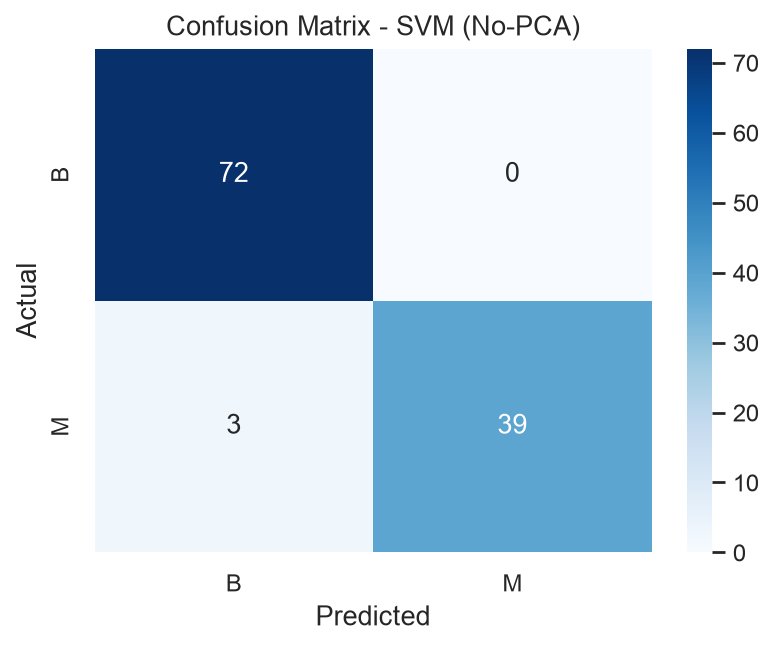
\includegraphics[width=\linewidth]{experiment7_output/plots/confusion_matrix_svm_no_pca.png}
\caption{SVM (No-PCA)}
\end{subfigure}
\hfill
\begin{subfigure}{0.24\textwidth}
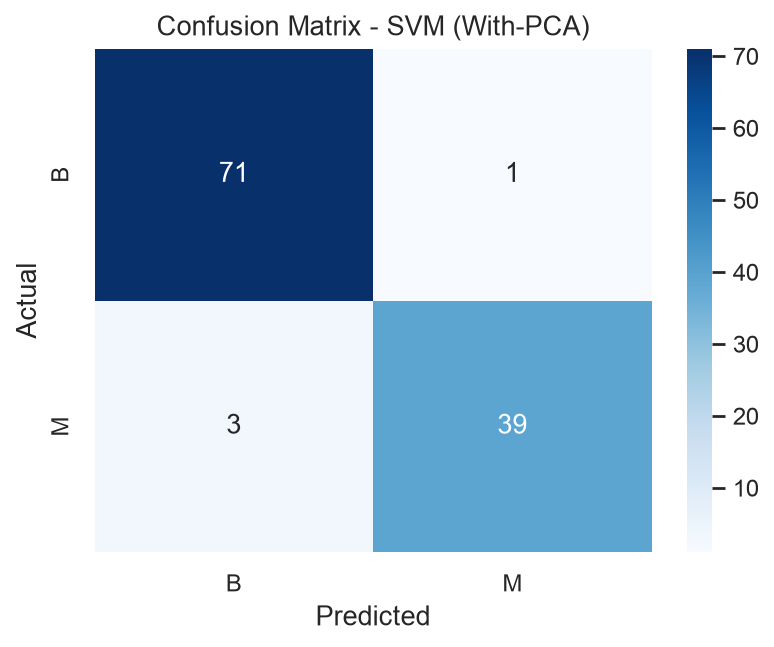
\includegraphics[width=\linewidth]{experiment7_output/plots/confusion_matrix_svm_with_pca.png}
\caption{SVM (With-PCA)}
\end{subfigure}
\hfill
\begin{subfigure}{0.24\textwidth}
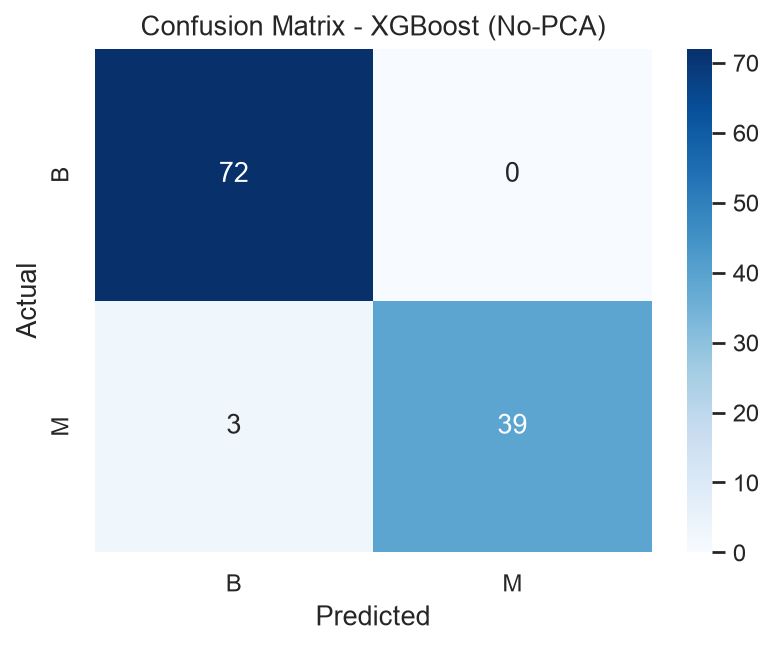
\includegraphics[width=\linewidth]{experiment7_output/plots/confusion_matrix_xgboost_no_pca.png}
\caption{XGBoost (No-PCA)}
\end{subfigure}
\hfill
\begin{subfigure}{0.24\textwidth}
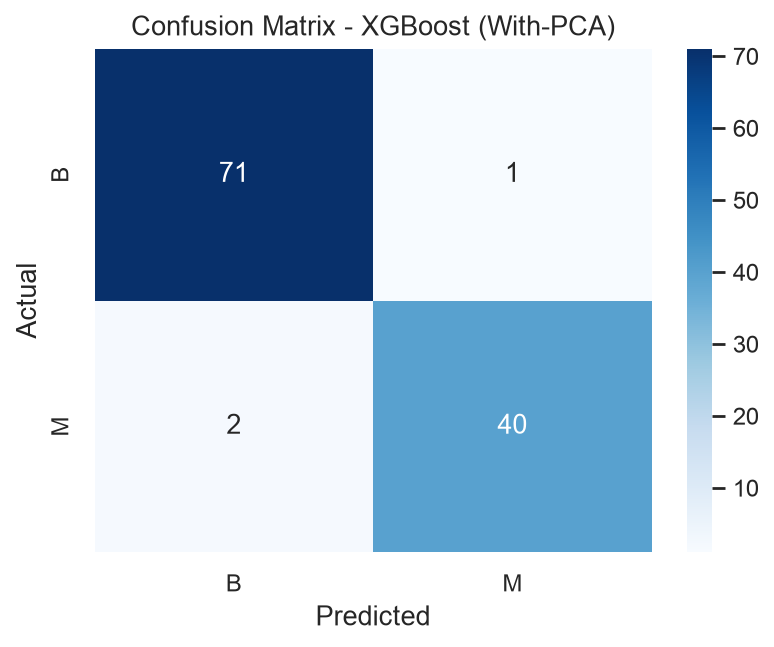
\includegraphics[width=\linewidth]{experiment7_output/plots/confusion_matrix_xgboost_with_pca.png}
\caption{XGBoost (With-PCA)}
\end{subfigure}
\caption{Confusion matrices, selected models (SVM and XGBoost), No-PCA vs.\ With-PCA.}
\end{figure}

\begin{figure}[h]
\centering
\begin{subfigure}{0.24\textwidth}
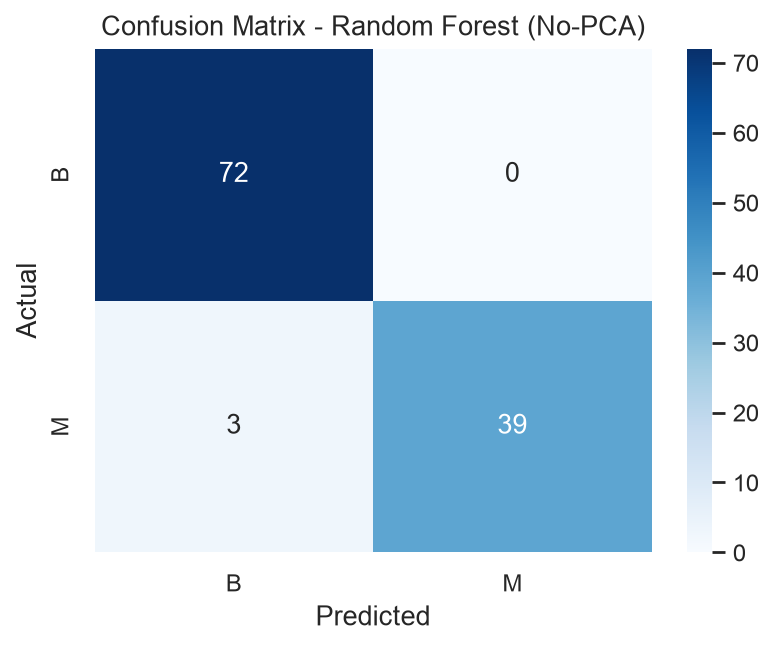
\includegraphics[width=\linewidth]{experiment7_output/plots/confusion_matrix_random_forest_no_pca.png}
\caption{Random Forest (No-PCA)}
\end{subfigure}
\hfill
\begin{subfigure}{0.24\textwidth}
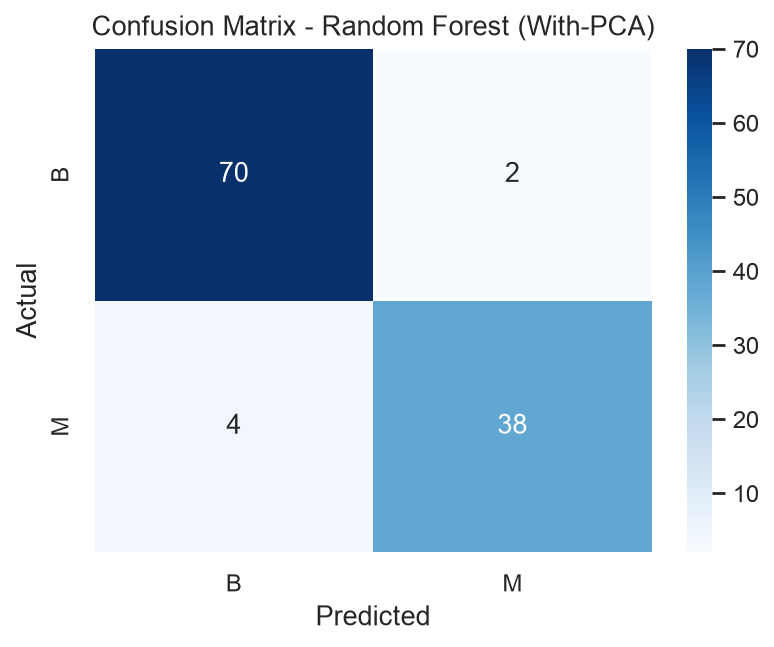
\includegraphics[width=\linewidth]{experiment7_output/plots/confusion_matrix_random_forest_with_pca.png}
\caption{Random Forest (With-PCA)}
\end{subfigure}
\hfill
\begin{subfigure}{0.24\textwidth}
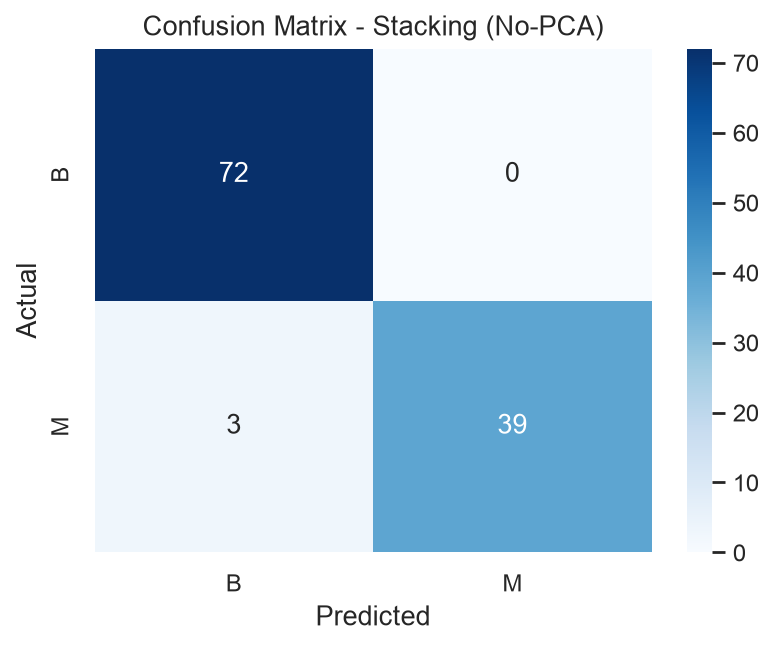
\includegraphics[width=\linewidth]{experiment7_output/plots/confusion_matrix_stacking_no_pca.png}
\caption{Stacking (No-PCA)}
\end{subfigure}
\hfill
\begin{subfigure}{0.24\textwidth}
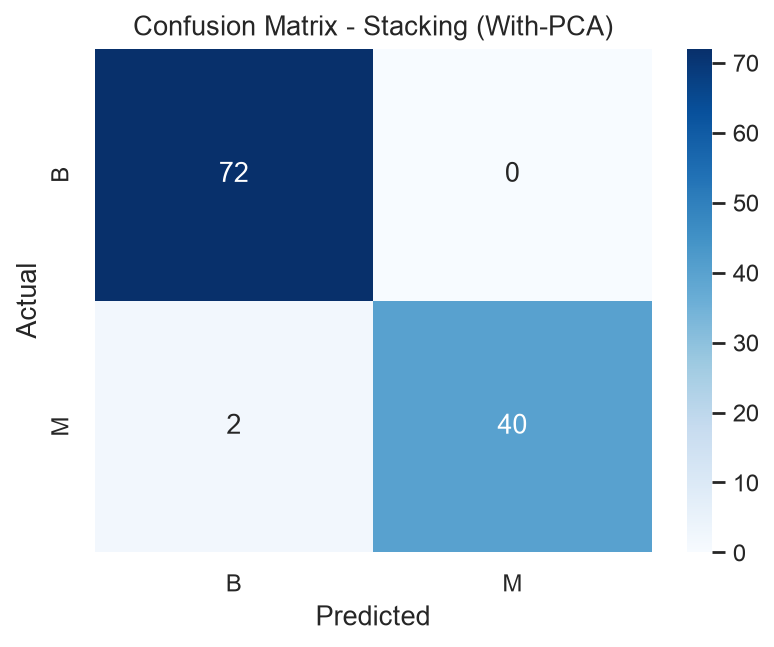
\includegraphics[width=\linewidth]{experiment7_output/plots/confusion_matrix_stacking_with_pca.png}
\caption{Stacking (With-PCA)}
\end{subfigure}
\caption{Confusion matrices, selected models (Random Forest and Stacking), No-PCA vs.\ With-PCA.}
\end{figure}
Stacking (With-PCA)'s confusion matrix shows only 2 misclassifications out of 114 test samples -- the fewest of any model/setting combination in this experiment -- consistent with it recording the highest test accuracy and F1 overall.

\begin{figure}[h]
\centering
\begin{subfigure}{0.48\textwidth}
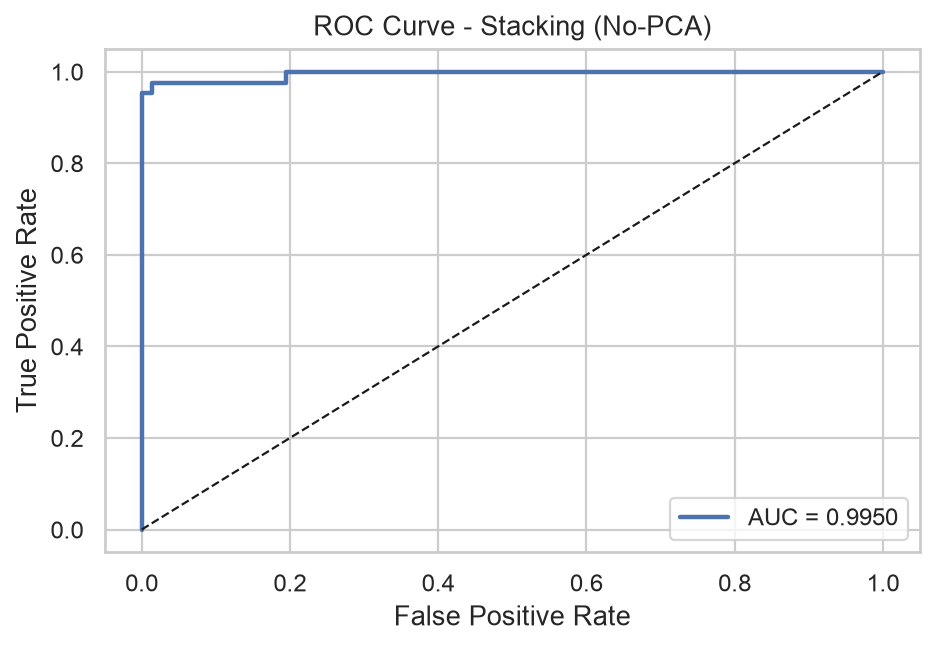
\includegraphics[width=\linewidth]{experiment7_output/plots/roc_curve_stacking_no_pca.png}
\caption{ROC, Stacking (No-PCA)}
\end{subfigure}
\hfill
\begin{subfigure}{0.48\textwidth}
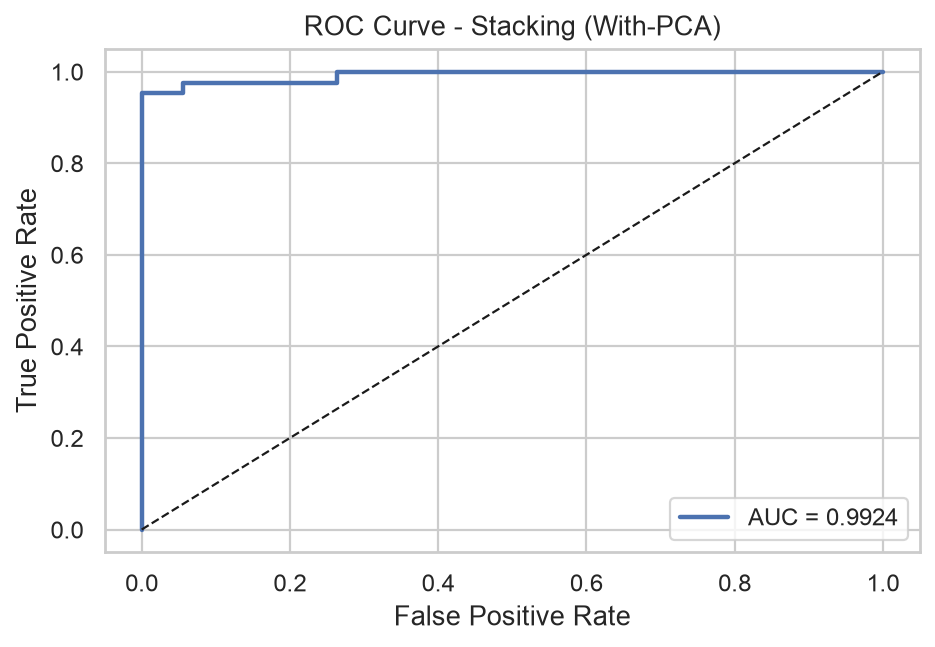
\includegraphics[width=\linewidth]{experiment7_output/plots/roc_curve_stacking_with_pca.png}
\caption{ROC, Stacking (With-PCA)}
\end{subfigure}
\caption{ROC curves for the Stacked Ensemble, No-PCA vs.\ With-PCA.}
\end{figure}

% ==========================================================
\section{PCA Impact Summary}
\begin{table}[h]
\centering
\small
\begin{tabular}{@{}lrrr@{}}
\toprule
Model & Accuracy Delta & F1 Delta & CV Fold-Std Delta (PCA $-$ No-PCA) \\
\midrule
Logistic Regression & +0.0088 & +0.0118 & +0.0027 \\
Stacking & +0.0088 & +0.0126 & $-$0.0032 \\
Decision Tree & 0.0000 & 0.0000 & $-$0.0162 \\
XGBoost & 0.0000 & +0.0009 & 0.0000 \\
SVM & $-$0.0088 & $-$0.0118 & +0.0050 \\
Gradient Boosting & $-$0.0088 & $-$0.0117 & $-$0.0006 \\
KNN & $-$0.0175 & $-$0.0250 & $-$0.0013 \\
Random Forest & $-$0.0263 & $-$0.0362 & $-$0.0020 \\
AdaBoost & $-$0.0263 & $-$0.0380 & $-$0.0058 \\
Naive Bayes & $-$0.0264 & $-$0.0318 & +0.0047 \\
\bottomrule
\end{tabular}
\caption{Test-set accuracy/F1 delta and CV fold-standard-deviation delta, With-PCA minus No-PCA, sorted by accuracy delta.}
\end{table}
Only Logistic Regression, Stacking, Decision Tree, and XGBoost show a non-negative accuracy delta under PCA; every other model loses accuracy, most severely Naive Bayes ($-$0.0264), AdaBoost ($-$0.0263), and Random Forest ($-$0.0263). This lines up closely with the theoretical expectation from Section 3.2: the two clearest winners are a linear model (Logistic Regression) and a meta-learner (Stacking) that can partially compensate for its base learners, while three of the four worst-affected models (Random Forest, AdaBoost) are tree ensembles whose split-based decisions are less compatible with a rotated PCA feature space.

% ==========================================================
\section{Observation Questions}

\textbf{Which models improved most with PCA? Which did not? Why?}\\
Logistic Regression improved the most with PCA on the test set (accuracy delta +0.0088), tied with Stacking (also +0.0088); Naive Bayes changed the least favorably, dropping by 0.0264. Logistic Regression is a linear model whose decision boundary is a hyperplane in feature space, so removing correlated, redundant directions via PCA sharpens that boundary without discarding useful signal, given that 10 components still retain 95.21\% of the variance. Naive Bayes, by contrast, depends on a per-feature independence assumption; while PCA should in principle make that assumption less wrong by decorrelating the input, in practice the 10 compressed components each mix information from many original features, which seems to have made the Gaussian per-component densities less separable rather than more, hurting Naive Bayes more than any other model tested.

\textbf{Did PCA reduce variance across folds (more stable results)?}\\
Averaged across all ten models, the 5-fold CV fold-to-fold standard deviation changed by only $-$0.0017 under PCA relative to No-PCA -- essentially a wash. The largest individual stabilization was on the Decision Tree, whose CV standard deviation fell from 0.0326 to 0.0164 (a 50\% reduction), which makes sense: a single tree's split choices are the most sensitive of any model here to which exact feature it happens to split on, and PCA's components, each blending several original features, give the tree fewer nearly-tied candidate splits to be unstable about. But this stabilizing effect did not generalize to the ensembles built on trees (Random Forest, AdaBoost both saw a modest CV standard-deviation reduction too, while Gradient Boosting and XGBoost were roughly flat), so PCA's variance-stabilizing effect on this dataset is real but narrow rather than universal.

\textbf{For high-dimensional data, was PCA beneficial in reducing overfitting?}\\
With only 30 original standardized features against 455 training rows, this dataset is not severely high-dimensional to begin with, so the overfitting-reduction case for PCA is inherently weak here -- and the results bear that out: half the models (SVM, Random Forest, AdaBoost, Gradient Boosting, KNN, Naive Bayes) lost test accuracy under PCA rather than gaining it, which would not happen if overfitting were the dominant effect being corrected. The one place PCA's dimensionality reduction clearly helped was cross-validation stability for tree-based models with high split-sensitivity (the Decision Tree, discussed above), rather than raw predictive accuracy.

\textbf{How did linear models (Logistic Regression, SVM) behave compared to ensemble models with PCA?}\\
Logistic Regression and SVM moved by an average accuracy delta of +0.0000 under PCA (Logistic Regression's +0.0088 gain almost exactly offsetting SVM's $-$0.0088 loss), versus $-$0.0153 for the four boosted/bagged tree ensembles (Random Forest, AdaBoost, Gradient Boosting, XGBoost). Even though the two linear/margin models did not move in the same direction as each other, their combined magnitude of change was far smaller than the ensembles', which is consistent with linear decision boundaries surviving an orthogonal rotation of the feature space more gracefully than axis-aligned tree splits do.

\textbf{Did stacking show robustness to dimensionality reduction compared to single models?}\\
Yes. Stacking's accuracy delta under PCA was +0.0088, better than the average absolute delta of 0.0137 across its three individual base models (SVM, Random Forest, Gradient Boosting), two of which (Random Forest, Gradient Boosting) actually lost accuracy under PCA. Stacking (With-PCA) also achieved the best overall test accuracy (0.9825) and F1 (0.9756) of any model or setting in this entire experiment, meaning the Logistic Regression meta-learner did not just average away its base learners' PCA sensitivity -- it turned two base learners' modest PCA-driven degradation and one base learner's PCA-driven improvement (SVM lost, but the ensemble still gained overall) into a net improvement, which is the practical payoff of training a meta-learner on out-of-fold predictions rather than simply voting.

% ==========================================================
\section{Discussion}
The central finding of this experiment is that PCA's effect is not a single yes/no answer but splits cleanly along model family lines: linear and meta-learner models (Logistic Regression, Stacking) were neutral-to-positive under PCA, while every tree-based ensemble except XGBoost (which was exactly flat) lost accuracy, and Naive Bayes -- despite PCA theoretically helping its violated independence assumption -- lost the most of any model. This is a more nuanced picture than either extreme ("PCA always helps by removing redundancy" or "PCA always hurts by discarding information"), and it matches the theoretical framing in Section 3.2 reasonably well for eight of the ten models; the two surprises are Naive Bayes' larger-than-expected loss and Stacking's larger-than-expected gain, both of which suggest that a model's behavior under PCA depends on more than just "is it distance-based or tree-based" -- Naive Bayes' loss likely comes from PCA components mixing away the very feature-level conditional structure Gaussian NB relies on, while Stacking's gain comes from the meta-learner's ability to reweight rather than simply average its base learners.

The main limitation, as in Experiments 5 and 6, is the small test set (114 rows), which makes small accuracy deltas (many in the 0.0088--0.0175 range) sensitive to a handful of flipped predictions rather than a robust population-level effect; the CV-based averages (Table 9) are more reliable evidence than any single test-set number. A second limitation specific to this experiment is that the same 95\%-variance PCA cutoff (10 components) was applied uniformly to every model, when in practice a model-specific search over the number of components (or over the variance target itself) might change some of the closer results, particularly for models like Random Forest and AdaBoost that lost the most accuracy under the fixed 10-component choice used here.

% ==========================================================
\section{Conclusion}
Ten classifiers were trained and hyperparameter-tuned on the Wisconsin Diagnostic Breast Cancer dataset, once on the original 30 standardized features and once on a 10-component PCA-reduced space retaining 95.21\% of the variance. The best No-PCA model was SVM (test accuracy 0.9737, F1 0.9630); the best With-PCA model, and the best model overall in this experiment, was the Stacked Ensemble (test accuracy 0.9825, F1 0.9756). PCA modestly helped linear/meta-learner models (Logistic Regression, Stacking) and left XGBoost and the Decision Tree essentially unchanged, but it hurt every other tree-based ensemble (Random Forest, AdaBoost, Gradient Boosting) and, most of all, Naive Bayes. The practical takeaway is that PCA is not a universally beneficial preprocessing step on this dataset: it is worth applying ahead of a linear model or as an input to a stacked ensemble's base learners, where a meta-learner can absorb any individual base learner's degradation, but tree-based ensembles trained directly on the well-behaved 30-feature space performed at least as well, and in most cases better, without it.

% ==========================================================
\section{References}
\begin{enumerate}[label={[\arabic*]}]
\item F. Pedregosa et al., ``Scikit-learn: Machine Learning in Python,'' \emph{Journal of Machine Learning Research}, vol. 12, pp. 2825--2830, 2011.
\item I. T. Jolliffe, \emph{Principal Component Analysis}, 2nd ed. Springer, 2002.
\item T. Chen and C. Guestrin, ``XGBoost: A Scalable Tree Boosting System,'' \emph{Proceedings of the 22nd ACM SIGKDD International Conference on Knowledge Discovery and Data Mining}, pp. 785--794, 2016.
\item D. H. Wolpert, ``Stacked Generalization,'' \emph{Neural Networks}, vol. 5, no. 2, pp. 241--259, 1992.
\item L. Breiman, ``Random Forests,'' \emph{Machine Learning}, vol. 45, no. 1, pp. 5--32, 2001.
\item W. H. Wolberg, W. N. Street, and O. L. Mangasarian, ``Breast Cancer Wisconsin (Diagnostic) Data Set,'' UCI Machine Learning Repository, 1995. [Online]. Available: \url{https://archive.ics.uci.edu/dataset/17/breast+cancer+wisconsin+diagnostic}
\item Scikit-learn Developers, ``Decomposing Signals in Components (PCA),'' \emph{Scikit-learn Documentation}. [Online]. Available: \url{https://scikit-learn.org/stable/modules/decomposition.html}
\end{enumerate}

\end{document}
